

\wwwcut{

\begin{table*}[t]
\centering
\resizebox{\textwidth}{!}{
\begin{tabular}{lrr}
\toprule
\textbf{Label}             & \textbf{Text Query}                                                                                                                                         & \textbf{URL Query}                                                                                                      \\
\midrule
BBBOnLine                  & (?:\textbackslash{}bBBBOnLine\textbackslash{}b|\textbackslash{}bBetter\textbackslash{}sBusiness\textbackslash{}sBureau\textbackslash{}b)                    & \textbackslash{}bbbb.org\textbackslash{}b                                                                               \\
DAA                        & (?:\textbackslash{}bDAA\textbackslash{}b|\textbackslash{}bDigital\textbackslash{}sAdvertising\textbackslash{}sAlliance\textbackslash{}b)                    & \textbackslash{}b(?:aboutads\textbackslash{}.(?:info)|digitaladvertisingalliance.org|youradchoices\textbackslash{}.com) \\
Web Beacon/Bug             & (?:web\textbackslash{}s(?:bug|beacon)|pixel)                                                                                                                &                                                                                                                         \\
Browser/Device Fingerprint & (?:browser|device)\textbackslash{}sfingerprint                                                                                                              &                                                                                                                         \\
BCR                        & \textbackslash{}b(?:BCR|Binding\textbackslash{}sCorporate\textbackslash{}sRules)\textbackslash{}b                                                           &                                                                                                                         \\
Yahoo/AOL                  & (?:\textbackslash{}bYahoo\textbackslash{}b|\textbackslash{}bAOL\textbackslash{}b|\textbackslash{}bAmerica Online\textbackslash{}b)                          & 136 URLs (omitted due to length)                                                                                        \\                             
\end{tabular}
}
\caption{A sample of the queries from Section \ref{subsec:trends}. URLs for Yahoo/AOL are omitted due to excessive length, but are of the form \texttt{\textbackslash{}b(?:url1|url2|...)\textbackslash{}b} }
\label{tbl:queries}
\end{table*}

}
\wwwcut{
\section{Parked domain\\ detection and removal}
\label{apd:parked-domain}

To remove policies from parked domains we first collected domain parking providers from prior research~\cite{vissers2015parking, kuhrer2014paint, kuhrer2014paint-TR, wang2006strider}. Then we considered the 10 registrars with the most first parties on the ICANN-Accredited Registrars list~\cite{ICANN-Registrars}, from which we manually reviewed ten samples. We found that six of these showed parked or expired domain pages, and four did not. We included the six that showed a parked page. Then we manually analyzed ten snapshots from the remaining top ten policy snapshot domains with most websites. We found that two were used exclusively for hosting domain parking service privacy policies and three were domain parking services or registrars. 
Our final list consisted of 79 parking providers and resellers.
}


\iffalse

\section{Text extraction benchmark}
\label{apd:text-extraction-benchmark}
\gnote{explain what this benchmark really measured, why we used a specific metric}
We decided on html2text after benchmarking different tools to extract text. We ran the benchmarks on 100 manually extracted policy texts as ground truth. Following Harkous et al.~\cite{harkous2018polisis}, we used a fuzzy text matching library~\cite{fuzzywuzzy} to score text similarity.
In total, we compared four different tools: 
three Python libraries (html2text~\cite{html2text-pypi}, Goose and lxml)
and a Linux command line utility (html2text).
We used each tool in two different modes:
\begin{enumerate*}[label=(\arabic*)]
\item directly extracting text from the saved policy web page,
\item extracting text from the readable version of the policy page.
\end{enumerate*}
We found that readable version, in combination with html2text Python library gives the best score (99\% median fuzzy match score, with an average of 92\%)\gnote{discuss the low scores}.
\fi

\wwwcut{\section{Manual analysis of crawl failures}
\label{apd:manual-err-verification}

We manually labeled 100 policies for each of the following conditions, to ensure the quality of our methods:

\textbf{No privacy policy link found on homepage.} 86 did not have a privacy policy anywhere on the site, based on our best efforts to find it. 4 had a privacy policy link on their homepage that we could not identify:  1/4 had a JavaScript popup link with an empty href element; 3/4 used a term that our link detection heuristics missed (e.g., ``Legal''). 2 had a policy link but it was image-based; the link contain no text that we could match against. 5 had a policy link on a different page than the homepage. 3 had no privacy policy link but the terms of service also contained the privacy policy.

\textbf{Detected as non-English.} 99 were non-English. 1 was a mixed language website with some English text.

\textbf{Detected as English.}  97 were only in English. 3 were mixed language with some English text.

\textbf{Policy page is not archived during interval.} 100 were not archived during the given interval.

\textbf{Blank homepage.} 65 were blank, i.e. contained no image or text. 13 were snapshots (median year=2001) that contained text, but they used a now obsolete ``<frameset>'' 
element to markup their pages. This caused our crawler to extract the text that is in a different frame than the top-level document. 19 were sites that were entirely composed of images, an early design pattern that lost its popularity due to limited accessibility. 3 were blank, but redirected to another page after a certain time; in one case to a live website that our crawler would block.
 }







\iffalse
\section{Readability}
\label{apd:readability_metrics}

The SMOG, Flesch-Kincaid, and Flesch ease reading scores determine the difficulty of reading text within the document. However, all three methods assume the text is written in the standard sentence structure typical of prose. Specifically, the Flesch-Kincaid and Flesch ease depend on the average number of words per sentence and average number of syllables per word, while the SMOG score depends on the average number of words with three or more syllables per sentence.
Therefore, in order to obtain accurate results, we removed non-sentence text
such as headers, tables, and lists by writing a custom Markdown renderer using Mistune~\cite{mistune} Markdown rendering library.

% FULL TEXT before trimming
The SMOG, Flesch-Kincaid, and Flesch ease reading scores determine the difficulty of reading text within the document. However, all three methods assume the text is written in the standard sentence structure typical of prose. Specifically, the Flesch-Kincaid and Flesch ease depend on the average number of words per sentence and average number of syllables per word, while the SMOG score depends on the average number of words with three or more syllables per sentence.
Therefore, in order too obtain accurate results, we removed non-sentence text. Examples of such text include headers, tables, and some lists. To accomplish this, we wrote a custom Markdown renderer using Mistune~\cite{mistune}, a Markdown rendering library, with the following behavior for these Markdown elements:
\begin{enumerate}
    \item For paragraphs and blocks of text, we render all complete sentences (defined as sequences of words that end with punctuation).
    \item For lists, we render each list item as a paragraph, and only render the list if all list items have at least one complete sentence.
    \item Links are rendered with either the link text if specified, otherwise the word ``link''.
    \item For most other types of elements (strikethrough, tables, and headings), we render nothing.
\end{enumerate}
We then take the output of this renderer and compute the scoring function of interest on it.

\fi

\rcut{
\section{Missing data}
\label{apd:missing}

As with many large-scale datasets, our dataset has missing data that should be considered, both in how it biases the data and how it affects analysis. 
%It is critical to consider missing data as we have no snapshots for \absentEngPerc\% of our candidate English websites as described in section \ref{sec:sec:building-website-list}.
There are four primary possible reasons a snapshot might be missing from our dataset. First, the website did not exist at the time. Second, the website existed, but did not have a privacy policy. Third, the Wayback Machine did not crawl the homepage or the privacy policy. Finally, our crawler could not find or download the privacy policy.

%The first and second reasons describe data that is non-existent, but is still worth considering -- our dataset will have more policies for websites that have existed for longer and had privacy policies. The third reason describes incomplete archiving. No archiving service can be complete, and our dataset inherits any biases from the Wayback Machine's archives. The final reason describes biases from our crawler; for example, our crawler may miss policies that do no use a standard link to direct users to their privacy policy. \rnote{should we cut this?}
The first and second reasons describe data that is nonexistent, which we still categorize as missing. The third reason describes incomplete archiving, for example due to crawl rules from \texttt{robots.txt}. The final reason describes biases from our crawler and classifier.
%; for example, our crawler may miss policies that do no use a standard link to direct users to their privacy policy. \rnote{should we cut this?}
}

%\label{apd:missing}

\wwwcut{
\begin{figure}[t]
\centering
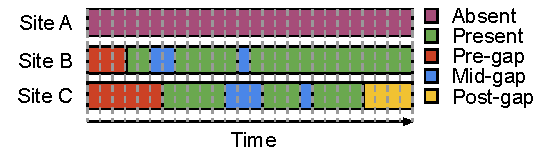
\includegraphics[width=\columnwidth]{figures/gaps_diagram.pdf}
\caption{An illustration of the 4 types of missing data. Here we have 3 sites: Site A never appears in our dataset; Site B's first snapshot appears early and has some missing snapshots; Site C's first snapshot appears later, it has some missing snapshots, and has missing snapshots after its last present snapshot}
\label{fig:missing_types}
\end{figure}
}

\rcut{
\textbf{Types of missing data.}
The categorization we use for the missing data is
illustrated in Figure \ref{fig:missing_types}. We categorize the missing data as ``absent'' and ``gap'', and further break down gaps as ``pre-'', ``post-'' and ``mid-gaps'' in the subsections below.

\textbf{Absent Data.} We categorize websites as absent if we have no privacy policies on any interval for that website. We find that \absentEngPerc\% of English websites as described in Section~\ref{sec:sec:building-website-list} are absent. We are more likely to have a privacy policy for a popular website: \absentEngOneKPerc\% of the English websites that have been in the Alexa Top 1K are absent.

\textbf{Gaps.}
%\gnote{86.1 of the snapshots do not have a gap between themselves and the previous snapshots from the same site. Let's not say midgaps are too common. And tell story from snapshots' point of view, not gaps. TODO: gunes rerun on non-dedup data}
%Once we remove all absent websites, the missing data that are left are gaps. 
%We think of gaps in terms of possible snapshots -- consider a matrix with one row per site and one column per interval, with a value of 1 if we have a privacy policy for that site-interval pair, and 0 if we do not. Each cell in this matrix is a possible snapshot.
%We find that, for non-absent websites, \gapsPerc\% of possible snapshots are a gap. Of these gaps, \pregapsPerc\% are pre-gaps, \midgapsPerc\% are mid-gaps, and \postgapsPerc\% are post-gaps. The large scale of pre-gaps is expected -- after all, most websites have not existed since 1997, and many websites are not archived by Internet Archive, especially before they gain popularity.
We categorize a snapshot as a gap
if we do not have a privacy policy in the snapshot's interval, but we do for a different interval for the same website.
We further break down gaps into `pre-gaps'', ``mid-gaps'' and ``post-gaps'' as illustrated in Figure~\ref{fig:missing_types}.
Even with perfect archiving, pre-gaps and post-gaps would still be expected, as websites come and go.
%Therefore, we believe mid-gaps to be the most important gaps to consider. 
A mid-gap, however, likely reflects a failure in archiving or collection rather than a lack of existence.
In our dataset, only \percSnapshotWithoutPrior\% of snapshots have a mid-gap immediately before them (i.e. a missing snapshot preceding a present snapshot that isn't the first snapshot for that interval), while 
%that are not the first snapshot for a site have another snapshot (i.e. do not have a mid-gap) immediately before them.
\midgapsDomainsPerc\% of websites have at least one mid-gap (i.e. a missing snapshot in any interval between the first and last present snapshots). Longer-lived websites are also more likely to have gaps---websites for which we have no gaps live an average \lifespanNoGaps~intervals, compared to \lifespanGaps~intervals for websites with gaps. Users of the dataset may consider imputing mid-gaps with a policy from a preceding or succeeding interval on the same website. The choice of which interval to draw from, and if imputation is needed, depends on the particular research question.
%A mid-gap likely reflects a failure in collection rather than a lack of existence. Thus, users of the dataset may consider imputing mid-gaps with a policy from a preceding or succeeding interval on the same website. The choice of which interval to draw from, and if imputation is needed, depends on the particular research question.]
}
\iffalse

Overall stats (e.g. perc of possible policies that are gaps)
Only do overall stats for websites that have a rank
Gap distribution based on w-i pairs with rank
% of websites that have pre/mid/post gaps?
Focus on mid-gaps, only briefly touch on pre/post gaps
median number of mid-gaps
Optional: how long do mid-gaps run?
Longevity: median(last\_year - start\_year)
\fi
%We categorize missing data into the following categories. 

\begin{comment}
For a missing snapshot, we categorize the missing data as follows (also illustrated in Figure \ref{fig:missing_types}):
\begin{itemize}
    \item ``absent'': We have no privacy policies on any interval for that website.
    \item ``gap'': We do not have a privacy policy for that snapshot, but we do for a different interval for the same website.
    \begin{itemize}
        \item ``pre-gaps'': We do not have a privacy policy for a prior interval, but we do for a later interval.
        \item ``mid-gaps'': We have a privacy policy for a prior and a later interval.
        \item ``post-gaps'': We have a privacy policy for a prior interval, but not for a later interval.
    \end{itemize}
\end{itemize}
\end{comment}

\rcut{
\textbf{Website popularity.}
We sought to determine if gaps are biased with respect to Alexa rank. For potential snapshots with a rank (rank $\leq$ 1M), we found the Pearson's correlation between Alexa rank and a binary gap variable to be \corrMidgap~ for mid-gaps, \corrPregap~for pre-gaps, and \corrPostgap~for post-gaps (p < 0.001). Among snapshots without a rank, just \midgapNoRankPerc\% of snapshots are mid-gaps, \pregapNoRankPerc\% are pre-gaps, \postgapNoRankPerc\%  are post-gaps, leaving just \notgapNoRankPerc\% of snapshots present. As we can see, mid-gaps do not seem to experience a noticeable bias with respect to rank, but pre- and post-gaps experience a small bias. However, pre- and post-gaps are strongly connected to being outside of the top 1M, supporting the hypothesis that pre- and post-gaps are partially caused by extremely low website popularity or non-existence. %\rnote{@AN is ``cause'' okay here?}
}
\iffalse
In order to identify if Alexa rank has any bias effects on gaps, we show how the percentage of snapshots that are gaps changes with rank in Figure \ref{fig:rank_absent}. We can see that pre-gaps and post-gaps are more common among high-ranked snapshots, whereas mid-gaps frequency does not seem to vary much with rank. Among snapshots without a rank, just \midgapNoRankPerc\% of snapshots are mid-gaps, \pregapNoRankPerc\% are pre-gaps, \postgapNoRankPerc\%  are post-gaps, leaving just \notgapNoRankPerc\% of snapshots present. This suggests that pre- and post-gaps are connected with a decline in rank, unlike mid-gaps, supporting the hypothesis that pre- and post-gaps are partially caused by low website popularity or non-existence.

\begin{figure}[t]
\centering
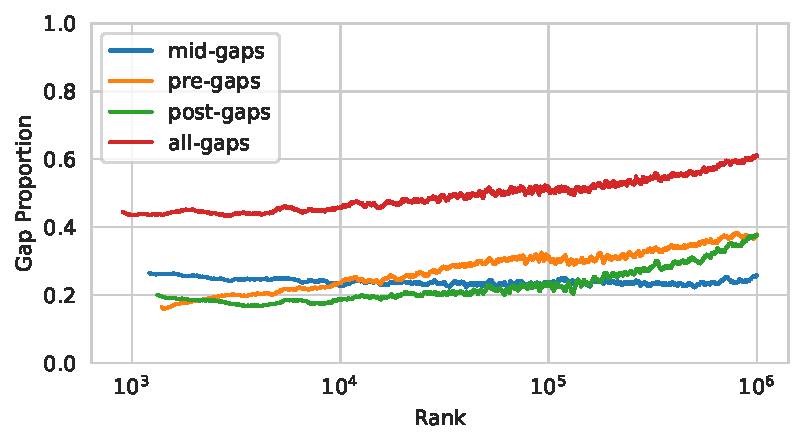
\includegraphics[width=1\columnwidth]{figures/gap_rank_absent.pdf}
\caption{The proportion of snapshots that are gaps as a function of rank. Proportion is calculated as the smooth moving average over the 10,000 neighboring snapshots. Snapshots without a rank are omitted. \rnote{Consider removal}}
\label{fig:rank_absent}
\end{figure}
\fi

% \begin{figure}[t]
% \begin{subfigure}[t]{0.45\textwidth}
% \centering
% 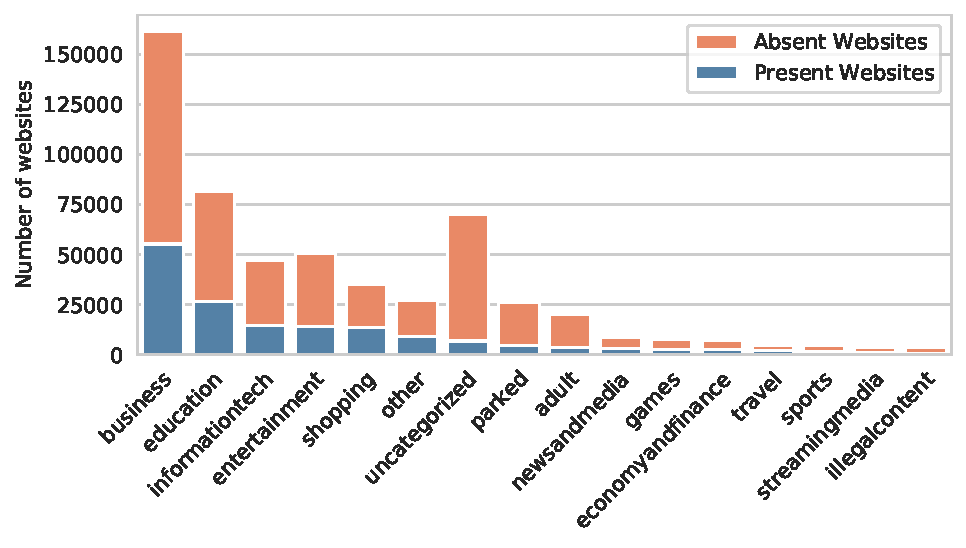
\includegraphics[width=1\columnwidth]{figures/category_dist.pdf}
% \caption{The distribution of website categories within our dataset.}
% \label{fig:cat_dist}
% \end{subfigure}
% \hfill
% \begin{subfigure}[t]{0.45\textwidth}
% \centering
% 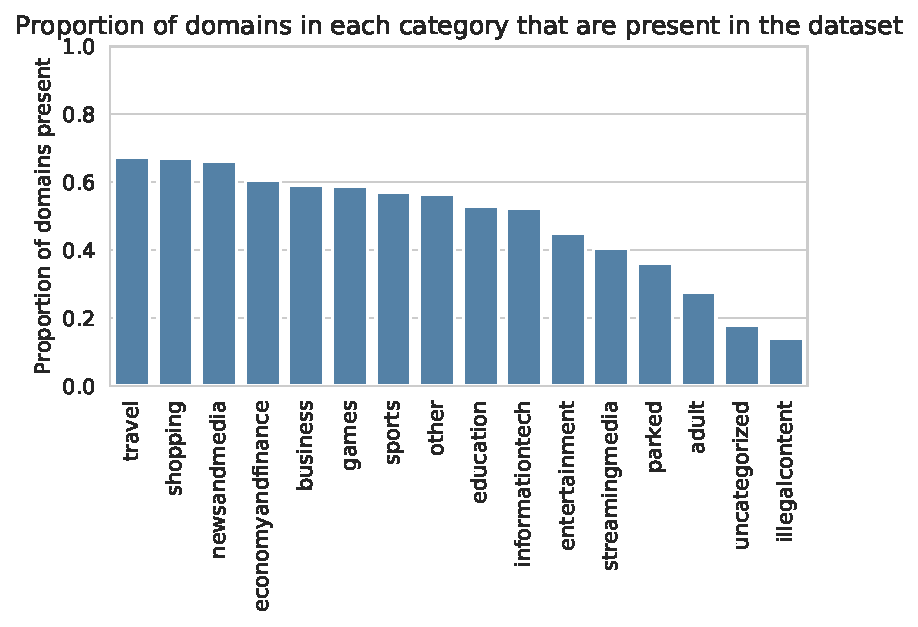
\includegraphics[width=1\columnwidth]{figures/category_missing_perc.pdf}
% \caption{The proportion of English-language websites for which we have privacy policies, grouped by category.}
% \label{fig:cat_prop}
% \end{subfigure}

% \caption{The representation of categories in our dataset. ``Other'' is composed of the 27 least frequent categories for English language websites. Policies which belong to multiple categories are counted once per category. Policies with no listed categories are added to the ``uncategorized'' category.\gnote{Think we should go back to the combined category plot or omit 6-b to save space. We can mention the uneven success across categories in the text}}
% \label{fig:categories}
% \end{figure*}
%\subsection{Evaluating data quality}
\label{subsec:ppot:failure-analysis}

To ensure our dataset was of high quality, we manually investigated causes of failure (i.e., homepages where the crawler did not extract privacy policy text). We started with 5,223,228 homepage snapshots, and our crawler was able to download 1,292,420 privacy policy snapshots (24\%).
Downloads of privacy policies corresponding to the other 3,930,808 homepage snapshots failed due to various causes which we list in Table~\ref{tab:failure-cause}. While the high frequency of absent policies may be counter-intuitive, we found that only about 2\% of missing policies were attributable to crawler limitations.

The most common cause for a missing privacy policy, by far, was the crawler loading an archived homepage but failing to identify a privacy policy link.
The next most common cause was a~\emph{blank homepage}, where the crawler could not extract any text. Another recurring issue was that, though we had attempted to filter our non-English sites before the crawl, some homepage snapshots were classified as non-English.

To investigate the root causes of crawler failures, we manually analyzed 100 random snapshots for each of the most common crawl failures.
The main takeaways are:
only 4 of 100 homepages where the crawler did not identify a privacy policy link actually had a privacy policy link. Only 3 of 100 homepages detected as \emph{blank} contained a privacy policy link, while 13 contained some text in a separate frame--- typically old webpages. We further explore the relation between the snapshot age and crawl success in 
Section~\ref{subsec:ppot:data-overview}.

In sum, the overwhelming majority of crawl failures were attributable to homepage snapshots that did not contain a policy link, were not archived by the Wayback Machine (e.g., due to \texttt{robots.txt} rules), or were in a language other than English. The missing privacy policies that are attributable to limitations of the crawler are about 2\% of all snapshots (4\% of 44.7\% + 3\% of 7.3\%).


\begin{table}[t]
\centering
\resizebox{0.9\columnwidth}{!}{%
\begin{tabular}{@{}lrr@{}}
\toprule
\textbf{Failure cause}                           & \textbf{Count} & \textbf{Percent} \\ \midrule
No privacy policy link found on homepage         & 2,336,849      & 44.7\%       \\
Homepage detected as blank                        & 383,337       & 7.3\%      \\
Non-English homepage                             & 310,563        & 5.9\% \\
Policy page is not archived in this interval     & 271,736        & 5.2\%\\
Out-of-interval redirection for homepage         & 158,727        & 3.0\%\\
\bottomrule
\end{tabular}%
}
\caption{The five most common causes for the crawler to not download a privacy policy for a homepage. Out-of-interval redirection (row 5) means our crawler was redirected by the Wayback Machine to a snapshot in a different interval.}
\label{tab:failure-cause}
\end{table}



\rcut{
\section{Monitoring market trends}
\label{apd:automated-trends}
\iffalse
\textbf{Cleaning.}\label{subsec:automated-trends-cleaning}
We expect that certain patterns are likely to change from policy to policy, even though they have the same semantic meaning. One example is the term ``please contact us at'' followed by an email address. In order to account for this, we replace URLs, email addresses, and named entities with placeholders. To detect URLs, we used the extraction methods described in Section~\ref{sec:policy-links}. To detect emails, we used the same technique, but with a different regular expression. To detect entities, we use named entity recognition (NER) to identify names of companies. We separately save named entities, emails, and URLs and treat them as a category of terms later in our processing. We restricted the policy set to only those policies between Jan, 2009 and December, 2019, because this is the period for which we have the highest quality data. With two intervals per year, this gives us 22 intervals of data.

After cleaning the data, we impute mid-gaps to be the closest, preceding snapshot.
\fi

\textbf{Term counting.}
\label{subsec:termcounting}
We expect that certain patterns are likely to change from policy to policy, even though they have the same semantic meaning. One example is the term ``please contact us at'' followed by an email address. In order to account for this we replace URLs, email addresses, and named entities with placeholders. Then we impute mid-gaps to be the closest, preceding snapshot.
We first break each document down into terms---n-grams and sentences. In terms of n-grams, we specifically examined 1,2,3, and 5-grams. Using \emph{NLTK}~\cite{nltk}, we constructed n-grams by first breaking the text into sentences, converting to lowercase, removing stopwords and words without alphabetic characters, then creating the n-grams. We also treated the URLs and NER entities as distinct types of terms. Because we are interested in the adoption of terms by parties, we count the document frequency of the terms. Missing policies that are not imputed do not contribute any terms.

\textbf{Term extraction.}
\label{subsec:termextraction}
We reduce the set of terms that could be of interest by finding terms that ever occur in at least 0.5\% of policies in a single interval, for performance reasons. To remove bias with respect to the number of policies in an interval, we normalize document frequency by the number of policies. We then score each term by the following metrics:
\begin{enumerate}
    \item \textbf{Variance} -- the variance of term count
    \item \textbf{Difference} -- The absolute value of the difference the count at the start interval and end interval
    \item \textbf{Gain} -- The difference between the count at the highest interval and the lowest interval
    \item \textbf{Loss} -- As in \textbf{Gain}, but negated
    \item \textbf{Sum} -- The sum of the counts in all intervals
    \item \textbf{Local Positive Slope} -- For two points with heights $A$, $B$, separated by $w$ intervals, the \textbf{Local Positive Slope} is $A-B$. We vary $w$ from $1$ to $5$.
    \item \textbf{Local Negative Slope} -- As in \textbf{Local Positive Slope}, but we compute $B-A$.
    \item \textbf{Spike} -- Peak prominence as implemented by \emph{SciPy}~\cite{scipy-prominence}.
    
    \iffalse For any local maximum with value $B$, with local minima $A,C$ to the left and right, we score the prominence as $B-max(A,C)$, as implemented in SciPy~\cite{scipy-prominence}. The \textbf{Spike} score is the maximum prominence over all local maxima.\fi
    
\end{enumerate}
For each term type and scoring metric, we record the top 50 terms for expert consideration.
% arxiv/camera ready to do:
%2020SciPy-NMeth
\iffalse
\section{Legitimate interests}\label{apd:legitimateinterests}
We found the following terms to be relevant to legitimate interests:
\begin{itemize}
    \item strategy
    \item products/services
    \item products/services develop
    \item fraud context
    \item experiences technical
    \item namely proper administration
    \item communications performance contract
    \item marketing communications performance
    \item managing business enable
    \item rights payment processing
    \item business conducting managing
    \item marketing strategy use
    \item research development market
    \item development market promote
    \item managing operating promoting
    \item operating promoting business
    \item best service/product best
    \item service/product best secure
\end{itemize}

\fi
}
\section{Privacy policy exclusion criteria}
\label{sec:labeling-criteria}
%\rnote{We should consider moving some of this to the appendix. We should also consider removing or moving the causes of failure from the definition. (could go in the appendix)}
%\gnote{I agree with moving to the appendix}

As described in Section~\ref{sec:sec:pp-definition}, we excluded documents from our corpus that met any of the following criteria.
%In this context, we limited ourselves to identifying policies as defined by each website: text that considered itself to be a privacy policy was considered a privacy policy. To identify a page that websites refer to as a privacy policy, we established a first definition during the crawl steps (Section \ref{sec:sec:download-policies}). The list of strings used in the crawls comes from prior research~\cite{libert2018automated} and from further manual analysis of websites from which we were not able to extract a privacy policy. %We leave it to the users to further filter the dataset in search for policies that satisfy their legal requirements.

%It is more natural to supplement our operational definition with what \textit{does not} constitute a privacy policy. Namely, a candidate document that meets \textit{any} of the following criteria is not a privacy policy:

%\item[Not about privacy] The document is not a legal document and does not contain disclosures about privacy practices on the website. Recall that the privacy policy link detection heuristic described in Section~\ref{sec:sec:download-policies} is designed to maximize recall rather than precision. Thus, links that do not lead to privacy policies could be detected and crawled as candidate policies if they contained text that matches our list of strings. For instance, in some websites
%a link with the text ``Security \& Policy'' leads to a privacy policy. In other pages, it leads to blog posts that the author categorized under ``Security \& Policy.'' Or, link texts that match our list may lead to web page snapshots that do not contain any main article text.
% \item The document is not a legal document and does not contain disclosures about privacy practices on the website. In our sample, these cases were easily identified manually because most of them resulted from links with anchored text containing the term ``privacy.'' These documents are crawled from unrelated web pages, such as pages discussing facts about privacy and security \gnote{Can you please help with this: "Explain why the prior validation might not catch this."}. In other cases, the links or snapshots of web pages do not contain text.
\textbf{Incomplete privacy policies.} The document contains an incomplete privacy policy.
\iffalse
In our sample, we found that this was linked either to incomplete text in the Wayback Machine snapshots, or to our text extraction module only storing part of the page text. 
The latter is caused by invalid HTML markup in the webpage, or an erroneous use of HTML tags, such as wrapping the privacy policy text in a \texttt{<footer>} element.
\fi
% GA: we've only 3 documents with partial text:
% one has text in a <footer> element, one has invalid HTML, the other has an incomplete WBM snapshot

\textbf{Terms of use and terms of service.} The document is a ``Terms of Use'' or a ``Terms of Service'' page, which might or might not contain a section dedicated to privacy.
%Approximately 2.5\% of the documents in the sample combine Terms of Service with the privacy policy. 
 \iffalse
Keeping hybrid documents that combine terms of use and privacy policy in the final dataset could potentially skew the results of trend analyses.
For example, considering these documents when analyzing longitudinal trends on the length of privacy policies can result in inaccuracies: these hybrid documents are long and would skew the results if used in their entirety. Furthermore, by marking these documents as belonging to the negative class, we reduce the number of false positives in our classification.
\fi

\textbf{Cookie Policies.} The document is a ``cookie policy''---that is, it only describes the behavior of the website in regards to cookies. 
\iffalse
Cookie policies are typically subsets of a privacy policy; however, we define a ``cookie policy'' as a document that \textit{only} describes cookies. 
\fi
%In our sample, fewer than 1\% of the documents adhere to this definition.

\textbf{Security policies.} The document is a ``security policy,'' which exclusively describes the security technologies employed by the website, such as the TLS.
\iffalse
These documents do not contain mentions of practices related to privacy.
\fi
%We found only one occurrence of a security policy in our sample.

\textbf{Mixed documents.} The document contains paragraphs that appear to be unrelated to a privacy policy. In other words, in order for a document to be classified as a privacy policy, every section of the document must be pertinent to privacy. 
\iffalse
This is, once again, a decision to reduce the number of false positives in our classification. Examples from our sample include mentions of the website's policy about copyrighted material.
\fi

\textbf{Privacy centers.} The document is a landing page that does not contain the privacy policy and, instead, only contains links to the privacy policy.

\textbf{Privacy policy summaries.} The document contains ``highlights'' of the privacy policy, often including a link to a complete version of the privacy policy.

\iffalse
\begin{table*}[t]
\centering
\resizebox{\textwidth}{!}{
\begin{tabular}{lrr}
\toprule
\textbf{Label}             & \textbf{Text Query}                                                                                                                                         & \textbf{URL Query}                                                                                                      \\
\midrule
BBBOnLine                  & (?:\textbackslash{}bBBBOnLine\textbackslash{}b|\textbackslash{}bBetter\textbackslash{}sBusiness\textbackslash{}sBureau\textbackslash{}b)                    & \textbackslash{}bbbb.org\textbackslash{}b                                                                               \\
TrustArc                   & (?:\textbackslash{}bTRUSTe\textbackslash{}b|\textbackslash{}bTrustArc\textbackslash{}b)                                                                     & \textbackslash{}btrust(?:e|arc)\textbackslash{}.(?:com|org)\textbackslash{}b                                            \\
DAA                        & (?:\textbackslash{}bDAA\textbackslash{}b|\textbackslash{}bDigital\textbackslash{}sAdvertising\textbackslash{}sAlliance\textbackslash{}b)                    & \textbackslash{}b(?:aboutads\textbackslash{}.(?:info)|digitaladvertisingalliance.org|youradchoices\textbackslash{}.com) \\
NAI                        & (?:\textbackslash{}bNAI\textbackslash{}b|\textbackslash{}bNetwork\textbackslash{}sAdvertising\textbackslash{}sInitiative\textbackslash{}b)                  & \textbackslash{}bnetworkadvertising\textbackslash{}.org\textbackslash{}b                                                \\
EDAA                       & (?:\textbackslash{}bEDAA\textbackslash{}b|European\textbackslash{}sInteractive\textbackslash{}Digital\textbackslash{}sAdvertising\textbackslash{}sAlliance) & \textbackslash{}b(?:edaa\textbackslash{}.eu|youronlinechoices\textbackslash{}.(?:eu|com))\textbackslash{}b              \\
Third Party                & third{[}\textbackslash{}-\textbackslash{}s{]}part(?:y|ies)                                                                                                  &                                                                                                                         \\
Cookies                    & \textbackslash{}bcookie                                                                                                                                     &                                                                                                                         \\
Web Beacon/Bug             & (?:web\textbackslash{}s(?:bug|beacon)|pixel)                                                                                                                &                                                                                                                         \\
Flash                      & flash                                                                                                                                                       &                                                                                                                         \\
Tracking technology        & tracking\textbackslash{}stechnolog(?:y|ies)                                                                                                                 &                                                                                                                         \\
"Evercookie                & evercookie                                                                                                                                                  &                                                                                                                         \\
Browser/Device Fingerprint & (?:browser|device)\textbackslash{}sfingerprint                                                                                                              &                                                                                                                         \\
Canvas Fingerprint         & canvas\textbackslash{}sfingerprint                                                                                                                          &                                                                                                                         \\
GDPR                       & (?:\textbackslash{}bDPR\textbackslash{}b|General Data Protection Regulation)                                                                                &                                                                                                                         \\
CCPA                       & (?:\textbackslash{}bCCPA\textbackslash{}b|California\textbackslash{}sConsumer\textbackslash{}sPrivacy\textbackslash{}sAct)                                  & https://oag\textbackslash{}.ca\textbackslash{}.gov/privacy/ccpa                                                         \\
COPPA                      & (?:\textbackslash{}bCOPPA\textbackslash{}b|Children.?s\textbackslash{}sOnline\textbackslash{}sPrivacy\textbackslash{}sProtection\textbackslash{}sAct)       &                                                                                                                         \\
CalOPPA                    & (?:\textbackslash{}bCalOPPA\textbackslash{}b|California Online Privacy Protection Act)                                                                      &                                                                                                                         \\
BCR                        & \textbackslash{}b(?:BCR|Binding\textbackslash{}sCorporate\textbackslash{}sRules)\textbackslash{}b                                                           &                                                                                                                         \\
SCC                        & \textbackslash{}b(?:Standard\textbackslash{}sContract(?:ual)?\textbackslash{}sClauses|SCC)\textbackslash{}b                                                 &                                                                                                                         \\
Privacy Shield             & Privacy\textbackslash{}sShield                                                                                                                              & privacyshield\textbackslash{}.gov                                                                                       \\
Safe Harbor                & Safe\textbackslash{}sHarbou?r                                                                                                                               & export\textbackslash{}.gov/safeharbor/                                                                                  \\
Yahoo/AOL                  & (?:\textbackslash{}bYahoo\textbackslash{}b|\textbackslash{}bAOL\textbackslash{}b|\textbackslash{}bAmerica Online\textbackslash{}b)                          & 136 URLs (omitted due to length)                                                                                        \\
Facebook                   & (?:\textbackslash{}bFacebook\textbackslash{}b)                                                                                                              & 26 URLs (omitted due to length)                                                                                         \\
Twitter                    & (?:\textbackslash{}bTwitter\textbackslash{}b)                                                                                                               & 12 URLs (omitted due to length)                                                                                         \\
Google                     & (?:\textbackslash{}bGoogle\textbackslash{}b|\textbackslash{}bDoubleclick\textbackslash{}b)                                                                  & 484 URLs (omitted due to length)                                                                                        \\
Amazon                     & (?:\textbackslash{}bAmazon\textbackslash{}b)                                                                                                                & 60 URLs (omitted due to length)                                                                                         \\
Automattic                 & (?:\textbackslash{}bAutomattic\textbackslash{}b)                                                                                                            & 14 URLs (omitted due to length)                                                                                         \\
Cloudflare                 & (?:\textbackslash{}bCloudflare\textbackslash{}b)                                                                                                            & 6 URLs (omitted due to length)                                                                                          \\
AppNexus                   & (?:\textbackslash{}bAppNexus\textbackslash{}b)                                                                                                              & 4 URLs (omitted due to length)          \\                                  
\end{tabular}
}
\caption{Table of queries. URLs for the third parties were omitted due to excessive length, but were of the form \texttt{\textbackslash{}b(?:url1|url2|...)\textbackslash{}b} \rnote{shrink}}
\label{tbl:queries}
\end{table*}
\fi
